It is fundamental in AVs to perceive the environment and understand the context in which the vehicle is operating for obvious reasons.
The perception system is responsible for collecting data from various sensors, such as cameras, LiDAR, radar, and ultrasonic sensors, to create a detailed representation of the vehicle's surroundings.
In this case, it is important to consider the possible tampering that can be done on these sensors to alterate the perception of the vehicle, leading to dangerous situations~\cite{kim2020cybersecurity, sec-sensors-2023, metro2020analysis, sensors}.

\subsection{Main sensors}\label{subsec:main-sensors}

\begin{enumerate}
    \item \textbf{Cameras}: Cameras are used to capture visual data, such as images and videos, of the vehicle's surroundings.
    \item \textbf{LiDAR (Light Detection and Ranging)}: LiDAR sensors use laser light to measure distances and create detailed 3D maps of the environment.
    \item \textbf{Radar (Radio Detection and Ranging)}: Radar sensors use radio waves to detect objects and measure their distance, speed, and direction.
    \item \textbf{Ultrasonic Sensors}: Ultrasonic sensors use sound waves to detect objects and measure their distance.
    \item \textbf{GPS (Global Positioning System)}: GPS sensors use satellite signals to determine the vehicle's location and navigate to a destination.
    \item \textbf{IMU (Inertial Measurement Unit)}: IMU sensors measure the vehicle's acceleration, orientation, and angular velocity.
\end{enumerate}

\begin{figure}[!htb]
    \centering
    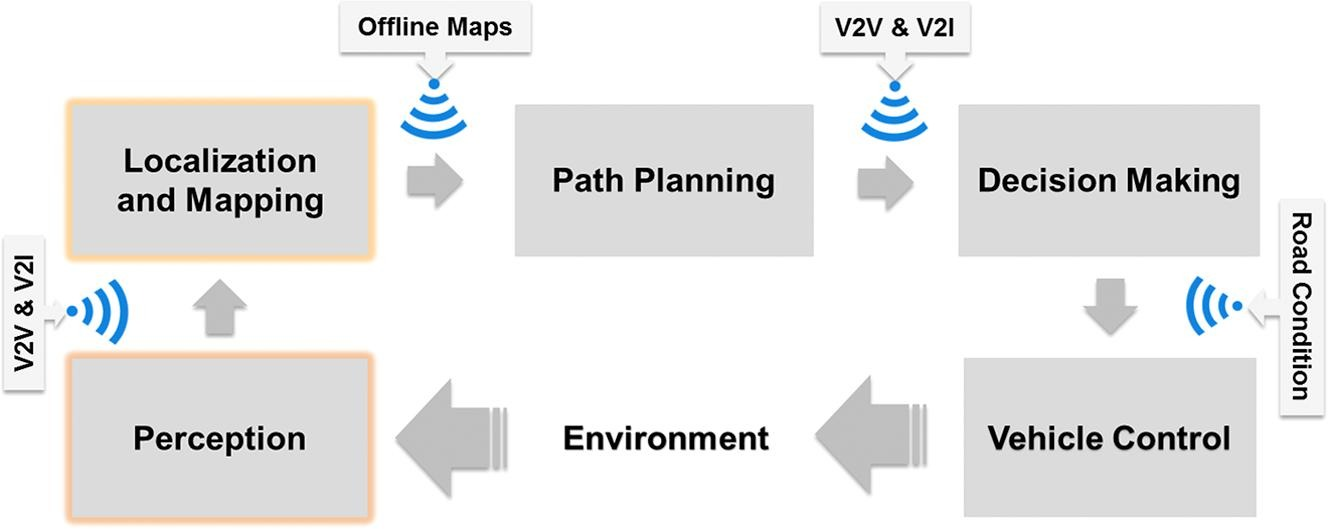
\includegraphics[width=0.7\linewidth]{figures/perception}
    \caption{Overview}
    \label{fig:sensors}
\end{figure}

As understood, these sensors provide the critical data needed for navigation, obstacle
detection, and decision-making processes and are essential for ensuring safety~\cite{unknown2020connected,cybersec}.

In the next sections~\ref{sec:cybersecurity-threats} there will be a deep dive into the main sensors used in AVs and their vulnerabilities.
